\documentclass[a4paper,11pt]{jsarticle}


% 数式
\usepackage{amsmath,amsfonts}
\usepackage{bm}
% 画像
\usepackage[dvipdfmx]{graphicx}


\begin{document}

\title{VSCodeで\LaTeX}
\author{Knfujioka}
\date{\today}
\maketitle

% 目次の表示
\tableofcontents
\section{セクション}
  ・・・
\subsection{サブセクション}
  ・・・
\subsubsection{サブサブセクション}
  ・・・
% --------------------------------------------------------

% 本文

\section{ロジスティックシグモイド}

式~(\ref{eq:sigmoid})の関数は標準シグモイド関数と呼ばれ、図~\ref{fig:sigmoid}のような形である。!!!~\ref{eq:alpha}!!


\begin{equation}
    \sigma(x) = \frac{1}{1 + exp(-x)}
    \label{eq:sigmoid}
\end{equation}

\begin{equation}
    \alpha = \frac{1}{x}
    \label{eq:alpha}
\end{equation}

\begin{figure}[htbp]
    \centering
    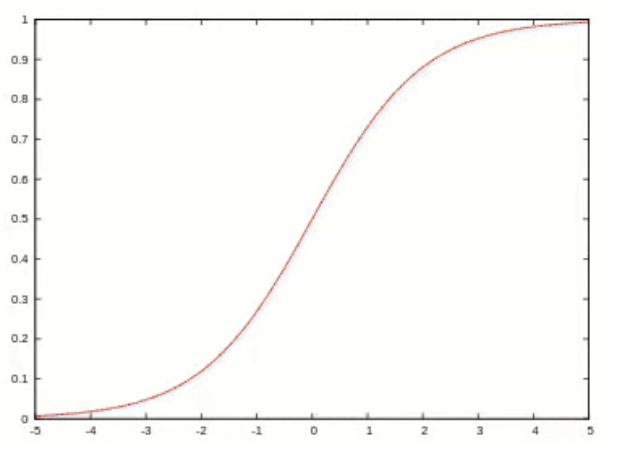
\includegraphics[width=8cm]{images/sigmoid.png}
    \caption{標準シグモイド関数}
    \label{fig:sigmoid}
\end{figure}

\newpage
\section{行列演算の基礎}

\begin{equation}
    \boldsymbol{w} = (\boldsymbol{X}^{T}\boldsymbol{X}^{-1})\boldsymbol{X}^{T}\boldsymbol{y}
\end{equation}

    \section{行列:演習問題}
    \centering
    $\boldsymbol{X} = \begin{bmatrix}
      1 & 2 & 3 \\
      1 & 2 & 5 \\
      1 & 3 & 4 \\
      1 & 5 & 9 \\
    \end{bmatrix}
    ,\ \boldsymbol{y} = \begin{bmatrix}
      1\\
      5\\
      6\\
      8\\
    \end{bmatrix}
    $
    \
    \
    \begin{flushleft}
      ()で書きたい場合。\\
      右揃え、左揃え、中央の書式について\\
      \underline{http://www.latex-cmd.com/struct/align.html}
    \end{flushleft}
    

    \[
        A = \left(
          \begin{array}{ccc}
            1 & 2 & 3 \\
            d & e & f \\
            g & h & i
          \end{array}
        \right)
    \]
    \begin{flushleft}
      行列式の書き方のフォーマット\\
      \underline{http://www.latex-cmd.com/equation/matrix.html} 
    \end{flushleft}

    \newpage
    \section{数列}
    \begin{equation}
      \sum_{x = 15}^{49} \frac{f(x)}{g(x)}
    \end{equation}
    \begin{flushleft}
    ・f(x):調査対象において、年齢xの女性が一年間に生んだ子供の数\\
    ・g(x):調査対象における、年齢xの女性の数
    \end{flushleft}

   \newpage
    \section{表}
      \subsection{罫線なしの表 (基本)}
    \begin{table}[htb]
      \begin{tabular}{lcrr}
        メニュー & サイズ & 値段 & カロリー \\
        牛丼 & 並盛 & 500円 & 600 kcal \\
        牛丼 & 大盛 & 1,000円 & 800 kcal \\
        牛丼 & 特盛 & 1,500円 & 1,000 kcal \\
        牛皿 & 並盛 & 300円 & 250 kcal \\
        牛皿 & 大盛 & 700円 & 300 kcal \\
        牛皿 & 特盛 & 1,000円 & 350 kcal
      \end{tabular}
    \end{table}

    \begin{flushleft}
      ・表に罫線を引く
    \end{flushleft}
    \begin{table}[htb]
      \begin{tabular}{|l|c|r||r|} \hline
        メニュー & サイズ & 値段 & カロリー \\ \hline \hline
        牛丼 & 並盛 & 500円 & 600 kcal \\
        牛丼 & 大盛 & 1,000円 & 800 kcal \\
        牛丼 & 特盛 & 1,500円 & 1,000 kcal \\ \hline
        牛皿 & 並盛 & 300円 & 250 kcal \\
        牛皿 & 大盛 & 700円 & 300 kcal \\
        牛皿 & 特盛 & 1,000円 & 350 kcal \\ \hline
      \end{tabular}
    \end{table}
\newpage
    \begin{flushleft}
      ・セルの結合\\
      ・水平方向 (列) にまたがる表
    \end{flushleft}
    \begin{table}[htb]
      \begin{tabular}{|l|c|r||r|} \hline
        \multicolumn{2}{|l|}{メニュー}
          & \multicolumn{1}{c||}{値段} & \multicolumn{1}{r|}{カロリー}\\ \hline \hline
        牛丼 & 並盛 & 500円 & 600 kcal \\
        牛丼 & 大盛 & 1,000円 & 800 kcal \\
        牛丼 & 特盛 & 1,500円 & 1,000 kcal \\ \hline
        牛皿 & 並盛 & 300円 & 250 kcal \\
        牛皿 & 大盛 & 700円 & 300 kcal \\
        牛皿 & 特盛 & 1,000円 & 350 kcal \\ \hline
      \end{tabular}
    \end{table}

    \begin{flushleft}
      ・セルの結合\\
      ・垂直方向 (行) にまたがる表
    \end{flushleft}
    \begin{table}[htb]
      \begin{tabular}{|l|c|r||r|} \hline
        メニュー & サイズ & 値段 & カロリー \\ \hline \hline
          & 並盛 & 500円 & 600 kcal \\ \cline{2-4}
        牛丼 & 大盛 & 1,000円 & 800 kcal \\ \cline{2-4}
          & 特盛 & 1,500円 & 1,000 kcal \\ \hline
          & 並盛 & 300円 & 250 kcal \\ \cline{2-4}
        牛皿 & 大盛 & 700円 & 300 kcal \\ \cline{2-4}
          & 特盛 & 1,000円 & 350 kcal \\ \hline
      \end{tabular}
    \end{table}

\newpage
\begin{flushleft}
  ・center 環境を使用した場合
\end{flushleft}
    % center 環境を使用した場合
\begin{table}[htb]
  \begin{center}
    \begin{tabular}{|l|c|r||r|} \hline
      メニュー & サイズ & 値段 & カロリー \\ \hline \hline
      牛丼 & 並盛 & 500円 & 600 kcal \\
      牛丼 & 大盛 & 1,000円 & 800 kcal \\
      牛丼 & 特盛 & 1,500円 & 1,000 kcal \\ \hline
    \end{tabular}
  \end{center}
\end{table}

\begin{verbatim}
  ・\centering コマンドを使用した場合
  入力通りの出力
  http://www.latex-cmd.com/struct/verb.html#verb
\end{verbatim}

% \centering コマンドを使用した場合
\begin{table}[htb]
  \centering
  \begin{tabular}{|l|c|r||r|} \hline
    メニュー & サイズ & 値段 & カロリー \\ \hline \hline
    牛丼 & 並盛 & 500円 & 600 kcal \\
    牛丼 & 大盛 & 1,000円 & 800 kcal \\
    牛丼 & 特盛 & 1,500円 & 1,000 kcal \\ \hline
  \end{tabular}
\end{table}

\newpage


\end{document}